Our preliminary testing focused on the raw, unprocessed accelerometer data from all three datasets. Our first goal was to replicate some of the standard machine-learning classifier results we found in previous literature \cite{ferrari2019hand}.

We initially wanted to confirm the results of training and testing on a raw data set \cite{ferrari2019hand}. We processed the data to be in the same format at the paper. The data was broken into 128-dimensional segments; there are 128 samples of each sensor (for each axes) within a single feature vector. In addition, each segment has a 50\% overlap with the previous feature vector. We ensured that the feature vectors were only made from data that was recorded consecutively, thus the overlap corresponded to their recording time. These vectors were created for each activity for each user in each of the datasets that we used, namely the Motion Sense and MobiAct datasets.

Our initial results were within one standard deviation of the results for the k-Nearest Neighbors (k-NN) and Support Vector Machine (SVC) classifiers \cite{ferrari2019hand}. Our results are summarized in Table~\ref{tab:ms} on the Motion Sense dataset and Table~\ref{tab:naive_mobi} on the MobiAct dataset. Our initial results were consistent with the results of previous studies in the instances of SVC and k-NN \cite{ferrari2019hand, he2016deep, ferrari2019homogenization}.  There was no overlap between the feature vectors in the train and test data sets. Notably, there has not been much interest in using the extra trees methods for classifying this type of data, despite our initial findings that it produces the best results and runs the fastest. 


\subsection{User Cross Validation}
\label{sub:user_cross_val}

For each dataset, we performed a cross validation across individual users in the dataset. In other words, for each user, we predicted their activity using a classifier trained on the data derived from all other uses. We believe that this is a better estimate of the robustness of the classification than a mixed or random training/test set because generally we cannot count on having prior examples of the behavior of persons whose behavior we wish to classify. The feature vectors consisted of only raw accelerometer data, as done in certain parts of \cite{ferrari2019hand}. We compared the results for the following classifiers: k-NN (3 nearest neighbors), SVC (using a one vs.\ rest scheme for more than two classes), and extra trees (100 estimators, minimum of 2 samples per split, and a minimum of 1 sample per leaf node).

\subsubsection{Motion Sense}
\label{sub:user_cross_val_motion_sense}
For the Motion Sense dataset, the extra trees classifier performed the best and had the lowest standard deviation of the three classifiers we tested. The SVC and k-NN performed about the same. The extra trees classifier was the best classifier for 70\% of the users. There was no readily apparent correlation between user features (height, weight, age, gender) and classifier performance. We looked at all six activities of daily life.

\begin{table}[H]
\caption{\textsc{Motion Sense}}
\label{tab:naive_classifiers}
\centering
\begin{tabular}{lccl||lccl}
\toprule
\multicolumn{1}{l}{\textbf{}} & \multicolumn{1}{c}{\textbf{SVC}} & \multicolumn{1}{c}{\textbf{k-NN}} & \multicolumn{1}{c}{\textbf{Trees}} & \multicolumn{1}{l}{\textbf{}} & \multicolumn{1}{c}{\textbf{SVC}} & \multicolumn{1}{c}{\textbf{k-NN}} & \multicolumn{1}{c}{\textbf{Trees}} \\ \midrule
\textbf{Mean}       & 73.4\%  & 73.8\%  & 83.3\%  &  
\textbf{SD}       & 10.3\% & 11.7\%  & 4.3\%     \\ \bottomrule
\end{tabular}
\label{tab:ms}
\end{table}


\subsubsection{MobiAct}
\label{sub:mobiact_init_res}
For the MobiAct dataset, the extra trees and k-NN performed similarity. We only looked at the following activities: jogging, sitting, standing, walking upstairs, and walking downstairs. For brevity, the only the mean and standard deviation results are shown in Table~\ref{tab:naive_mobi}. While only doing the bare minimum data processing as described in Sec.~\ref{sub:data_proc}, we ran simple classifiers on the raw accelerometer data. Our k-nearest neighbors and extra trees classifiers performed comparably to the Motion Sense data and our results were within a standard deviation of the results found in other literature \cite{ferrari2019hand}. 

\begin{table}[H]
\caption{\textsc{MobiAct}}
\label{tab:mobiact-naive}
\centering
\begin{tabular}{lccl||lccl}
\toprule
\multicolumn{1}{l}{\textbf{}} & \multicolumn{1}{c}{\textbf{SVC}} & \multicolumn{1}{c}{\textbf{k-NN}} & \multicolumn{1}{c}{\textbf{Trees}} & \multicolumn{1}{l}{\textbf{}} & \multicolumn{1}{c}{\textbf{SVC}} & \multicolumn{1}{c}{\textbf{k-NN}} & \multicolumn{1}{c}{\textbf{Trees}} \\ \midrule
\textbf{Mean}       & N/A  & 92.19\%  & 94.09\%  &  
\textbf{SD}       & N/A & 12.20\%  & 13.89\%     \\ \bottomrule
\end{tabular}
\label{tab:naive_mobi}
\end{table}



\begin{figure}[H]
\begin{subfigure}{.5\textwidth}
  \centering
    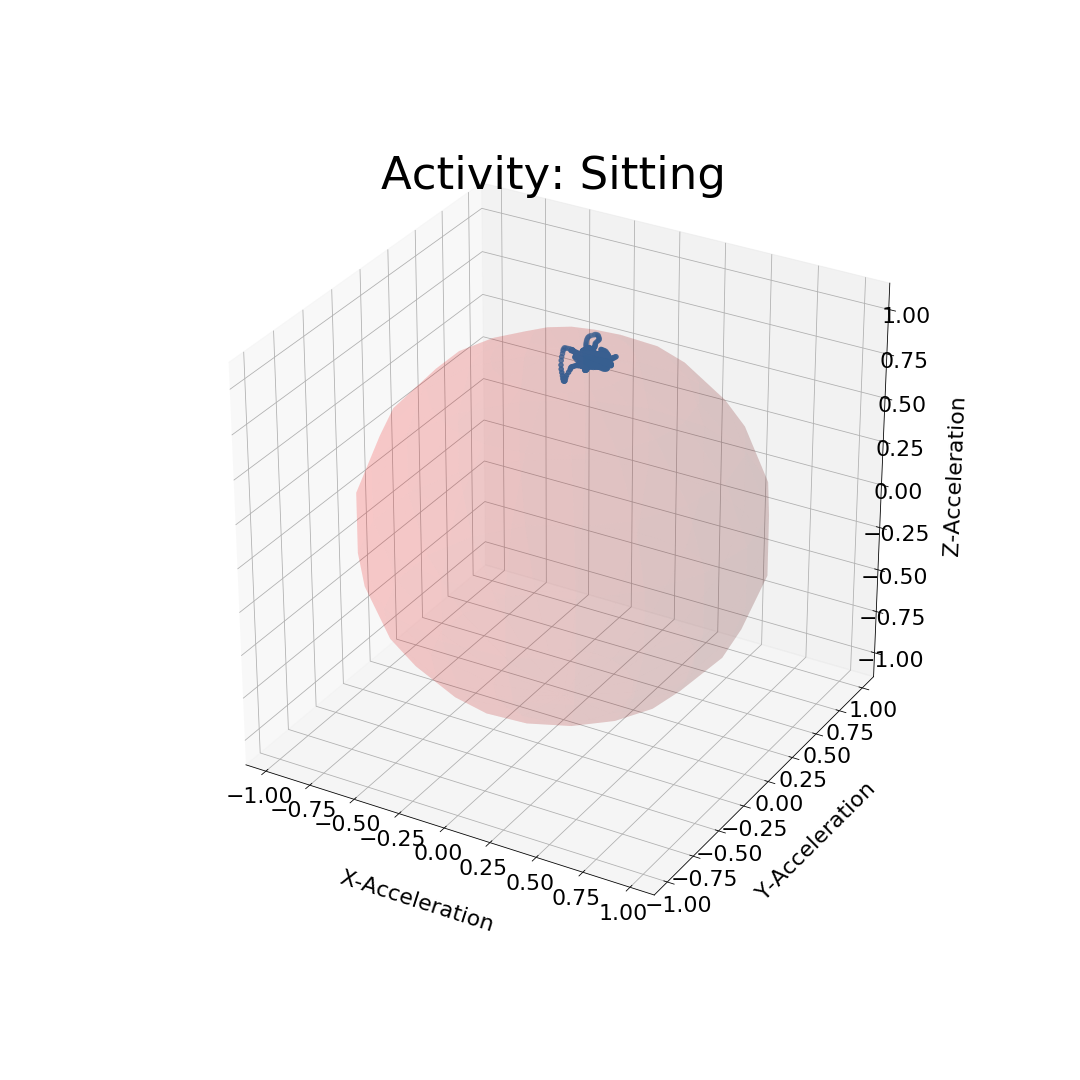
\includegraphics[width = \textwidth]{images/mobiAct/sitting.png}
    \caption{Mobi Act Dataset}
    \label{fig:mobiAct_sitting_comp}
\end{subfigure}
\begin{subfigure}{.5\textwidth}
  \centering
  % include second image
  \centering
  \includegraphics[width=\linewidth]{images/motionSense/Sitting_user_3.png}  
  \caption{Motion Sense Dataset}
  \label{fig:motionSense_sitting_comp}
\end{subfigure}
\caption{The images above were made for a random user in each dataset. As can be seen, there is significant difference in the clustering of the acceleration data between the two datasets used. The direction of the given acceleration vector $\vu a$ is mapped to $(x,y,z)$ and is plotted on the spheres.}
\label{fig:sitting_comp}
\end{figure}

\subsection{Visualization}
\label{sub:visual}
To move towards new representations of our data, we investigated different visualizations.

For the first visualization in Figure~\ref{fig:mobiAct_sitting_comp}, we plotted the direction of accelerometer $(x,y,z)$ observations onto the surface of a sphere. A comparison was made for the sitting patterns of a random user from both the MobiAct and Motion Sense datasets.  Comparing the two (Figs.~\ref{fig:mobiAct_sitting_comp}~and~\ref{fig:motionSense_sitting_comp}), the Motion Sense data is consistent with what we might expect from the waist/torso of someone who is sitting in a chair---the accelerometer data is predominately located at the poles ($z$-acceleration) as someone might shift her weight back and forth. In contrast, the MobiAct data features a much tighter distribution that is suggestive of the very small side to side back and forth that a phone may experience in the front pocket of a pair of pants. In this case, a rotationally invariant representation of the data would not resolve the inconsistency. These would be two different modes of sitting that would require distinct training examples to predict. Surprisingly, both datasets recorded data from the users' front pocket. Despite the same location on the user, the images look nothing alike. 

\begin{figure}[H]
\begin{subfigure}{.5\textwidth}
  \centering
    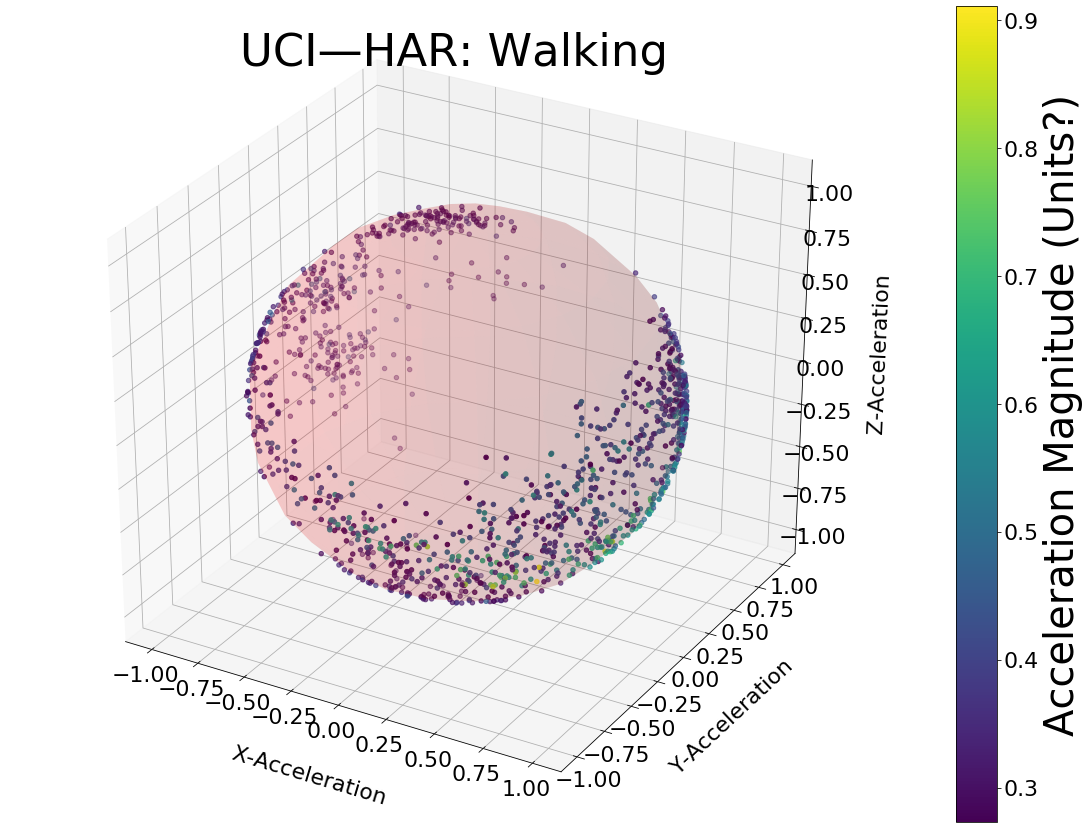
\includegraphics[width = \textwidth]{images/UCI_HAR/color_walking.png}
    \caption{Walking.}
    \label{fig:uci_walking}
\end{subfigure}
\begin{subfigure}{.5\textwidth}
  \centering
  % include second image
  \centering
  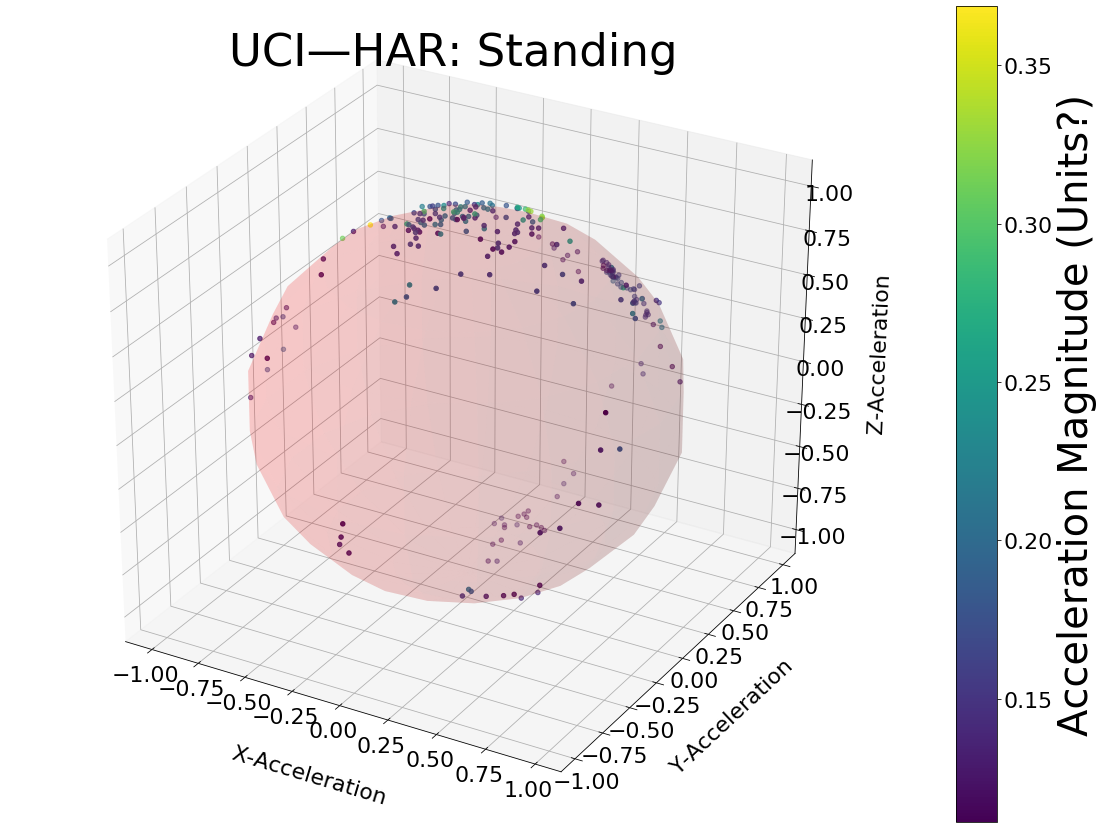
\includegraphics[width=\linewidth]{images/UCI_HAR/color_standing.png}  
  \caption{Standing.}
  \label{fig:uci_standing}
\end{subfigure}
\begin{subfigure}{0.5 \textwidth}
  \centering
  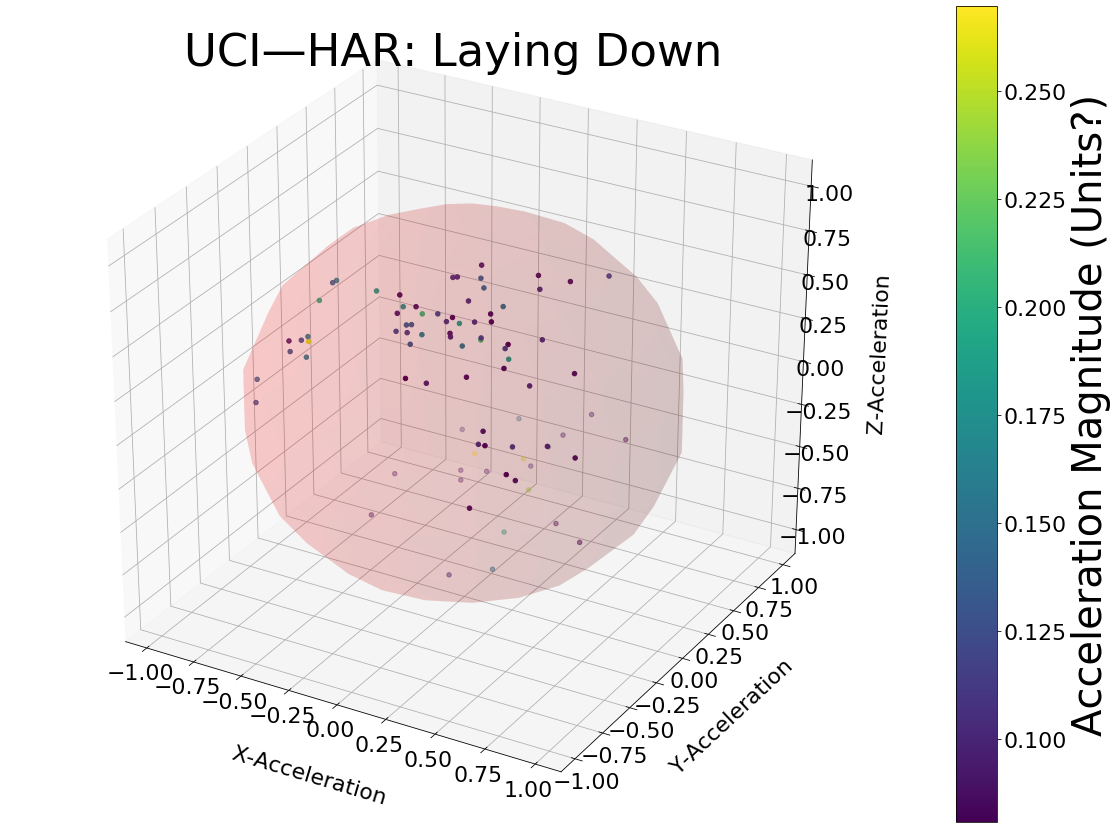
\includegraphics[width=\linewidth]{images/UCI_HAR/color_laying.png}  
  \caption{Laying.}
  \label{fig:uci_laying}
\end{subfigure}
%
% fourth image
\begin{subfigure}{0.5 \textwidth}
  \centering
  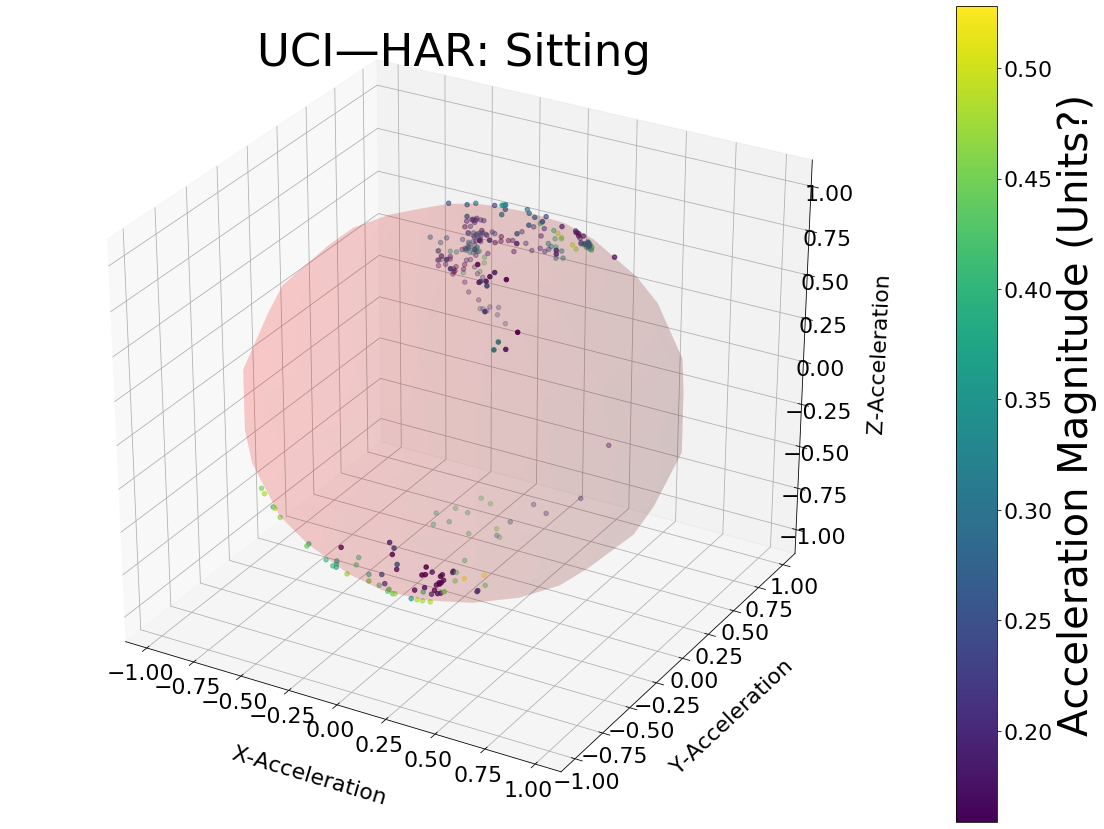
\includegraphics[width=\linewidth]{images/UCI_HAR/color_sitting.png}  
  \caption{Sitting.}
  \label{fig:uci_sitting}
\end{subfigure}
%%
%%
\caption{The direction and magnitude acceleration measured by the phone's accelerometer plotted on the surface of a unit sphere with the much of the low magnitude noise filtered out. The point on the sphere describes the $x$-,$y$-,$z$-direction of the vector itself. By filtering, we can remove much of the noise. For example, laying down has points scattered all around the surface of the sphere, essentially random whereas the sitting has accelerations on two opposite poles, suggesting a small adjustment (e.g.\ the shifting of a leg). More active movements like walking trace out arcing paths along the surface of the sphere.}
\label{fig:uci}
\end{figure}



Second, we performed a similar visualization, separating based on the labeled activity within the UCI dataset for the same user as in Figure~\ref{fig:sitting_comp}. Again, the direction of the given acceleration vector $(x,y,z)$ was plotted on a unit sphere, plus each point was colored to represent the magnitude of the acceleration. Only points with a magnitude of at least 30\% of the maximum magnitude value was shown. This was a completely arbitrary value, however it allows us to get rid of much of the noise associated with the data and to more clearly see the trends of each activity. The sitting data is again consistent with the swaying back and forth of a torso while sitting in a chair. The standing data appears to show that the strongest acceleration occurs swaying side to side. The walking data appears clustered around a ring in the center of the sphere, possibly reflective of this individual's stride. Lastly, the laying down is difficult to interpret, although appears to show few data points with large accelerations. However, if you note the scale bar, it is significantly lower than any of the other activities of daily life. 


The next visualization that was performed involves the time-integration of the accelerometer data which gives a proxy for the phone's velocity as a function of time. We can integrate again to get a proxy for the phone's position as a function of time. Figure~\ref{fig:motionSense_grid} provides a nice example of this below. Compare the parameterized velocity curves for jogging and walking. The walking velocity quite clearly shows a downward drift in the velocity. We suspect this is an artifact of either the sensor or our current data analysis, as the velocity of a phone in a front pocket should not have systematic decrease over the course of a few seconds. Another important feature of the velocity parameterization of jogging(and less obviously in the walking data) is the sharp, periodic, looping structure. 

An interesting observation to note in the jogging data is that over the course of the \SI{2.56}{\s}, the velocity curve has nearly three full repetitions. This is a well-known characteristic of running cadence where a runner is expected to take 150--180 steps per minute \cite{interview}. Our intuition tells us that we should expect a somewhat coiled velocity that is quasi-periodic, which can be achieved if we can eliminate or mitigate the drift. Regardless, these nearly periodic coils provide a strong signal for a phone's movement over short time frames.

\begin{figure}[ht]
\centering
\includegraphics[width=1. \textwidth]{images/motionSense/full_grid.png}  
\caption{A \SI{2.56}{\s} window of accelerometer data (obtained at \SI{50}{\Hz}) from User 1 in the Motion Sense dataset is examined for jogging, walking, and sitting. The direction of acceleration is shown in the top row, a velocity obtained from integrating the acceleration (with $\vb v(0) = (0,0,0)$) is shown in the middle row, and a position obtained from integrating the velocity is shown in the bottom row (with $\vb x(0) = (0,0,0)$). Each component of acceleration is smoothed using a Gaussian filter with $\sigma = \SI{0.04}{\s}$ to reduce high-frequency noise. For each entry, time is implicitly represented using a jet color map going from blue (beginning) to green (middle) to red (end).}
\label{fig:motionSense_grid}
\end{figure}


\begin{figure}[ht]
\centering
\includegraphics[width=1. \textwidth]{images/motionSense/acceleration_grid.png} 
\caption{A \SI{2.56}{\s} window of accelerometer data (obtained at \SI{50}{\Hz}) from is examined for jogging, walking, and sitting. The $x$-, $y$-, and $z$-components of acceleration are shown separately and smoothed using a Gaussian filter with $\sigma=\SI{0.04}{\s}$.}
\label{fig:motionSense_acc_grid}
\end{figure}

Finally, in Figure ~\ref{fig:motionSense_acc_grid}, we examined the $x,y,$ and $z$ components of the accelerometer data separately for the same \SI{2.56}{\s} window as Figure~\ref{fig:motionSense_grid}. Again, the individual accelerations are smoothed using a Gaussian filter with $\sigma=\SI{0.04}{\s}$ to eliminate high frequency noise. The acceleration for the jogging and walking segments much more clearly reflects the inherently periodic nature of these movements than the direction of acceleration plotted in three dimensions in Figure~\ref{fig:motionSense_grid}. The user appears to undergo about 3.5 cycles of movement in the jogging data and 2.5 cycles in the walking. By contrast, the sitting data does not appear to have a clear periodic structure. Furthermore the amplitude of the accelerations during jogging and walking are orders of magnitude greater than that experienced during the sitting ($\sim 1$ vs.\ $\sim 0.01$).

